\section{Empirical Signatures}\label{sec:signatures}

% Role: testable predictions that separate offsetting entry from pure displacement, each mapped to data.

The model implies a set of predictions that distinguish two hypotheses.
Under \emph{pure displacement}, AI lowers employment at large incumbents with no offsetting response at the entry margin.
Under \emph{offsetting entry}, the same shock also lowers the cost of starting and running a firm, so entry and employment in the band $\Bc$ rise in AI-exposed industries.
Each prediction below is stated relative to less-exposed industries in the same country and year.

\begin{prediction}[Incumbent headcount]\label{pred:incumbent}
Employment at firms that were large before the shock falls in AI-exposed industries.
This prediction holds under both hypotheses and serves as a check that the exposure measure captures the displacement channel.
\end{prediction}

\begin{prediction}[Entry]\label{pred:entry}
Firm entry rates rise in AI-exposed industries relative to their pre-shock trend.
Under pure displacement, entry does not respond, or falls if displaced workers face weaker demand for their skills.
\end{prediction}

\begin{prediction}[Entrant size]\label{pred:entrant-size}
Average employment at entry falls, because the AI task share $\phi$ also applies to entrants, while the number of entrants rises.
\end{prediction}

\begin{prediction}[Employment in the band]\label{pred:band}
Employment at firms in the band $\Bc$, classified by pre-shock size and including entrants, rises in AI-exposed industries.
The offset ratio $\Omega$ in \cref{eq:offset-ratio} is the ratio of this response to the response in \cref{pred:incumbent}.
\end{prediction}

\begin{prediction}[Capital required at entry]\label{pred:capital}
The amount of external capital raised before a firm's first product falls in AI-exposed sectors, by analogy with the cloud era \citep{ewens2018cost}.
\end{prediction}

\begin{prediction}[Transatlantic differences]\label{pred:us-europe}
The employment response in the band $\Bc$ is larger in the United States than in Europe, and the gap appears mainly in the post-entry growth of AI-exposed entrants rather than in entry rates.
Europe's employer start-up rate is about half the US rate, its employment protection is about three times as strict, and its private AI investment is roughly a tenth of the US level; formal start-up registration costs, by contrast, are not systematically higher \citep{eurostat2026bdsize,oecd2020epl,oecd2024pmr,hai2026aiindex}.
The AI Act raises fixed compliance costs for entrants in high-risk uses \citep{euaiact2024}.
In a stylized European parameterization of the Monte Carlo (\cref{sec:disc-europe}), the probability of offset falls from 82\% to 70\%, mostly through thinner scale-up finance for AI-native entrants rather than through entry costs.
The transatlantic difference remains smaller than the uncertainty in $\sigma_{\text{ai}}$ (\cref{tab:sensitivity}).
\end{prediction}

\Cref{tab:signatures} maps each prediction to candidate US and European data sources.

\begin{table}[t]
  \centering
  \caption{Empirical signatures and candidate data sources}
  \label{tab:signatures}
  \begin{tabular}{lll}
    \toprule
    Prediction & United States & Europe \\
    \midrule
    \ref{pred:incumbent}.\ Incumbent headcount & BDS; BTOS (Oct 2026: 2\% cut) & Community Survey on ICT \\
    \ref{pred:entry}.\ Entry & BFS (2025: +62\% vs.\ 2019) & Eurostat business demography \\
    \ref{pred:entrant-size}.\ Entrant size & BDS; BFS (WBA share 2026: 6.8\%) & OECD DynEmp \\
    \ref{pred:band}.\ Band employment & Business Dynamics Statistics & Eurostat SBS \\
    \ref{pred:capital}.\ Capital at entry & PitchBook, Crunchbase & Dealroom \\
    \ref{pred:us-europe}.\ Transatlantic gap & \multicolumn{2}{c}{Harmonized via OECD DynEmp} \\
    \bottomrule
  \end{tabular}
  \par\smallskip
  \parbox{\linewidth}{\footnotesize BFS figures from \citet{bfs2026}: business applications in 2025 relative to 2019, and applications with planned wages (WBA) as a share of all applications, January--September 2026. BTOS figure from \citet{btos2026oct}.}
\end{table}

\paragraph{AI exposure measure.}
We measure AI exposure at the industry level using task-based scores from \citet{eloundou2024gpts} and \citet{felten2021occupational}, mapped to NAICS (US) and NACE (Europe) via crosswalks.
\placeholder{Report the range of industry exposure scores once the crosswalk is computed. The simulation uses relative exposures of 0.5 (goods production), 0.8 (trade and transport), 1.2 (professional services), and 1.5 (information and finance), an ordering consistent with AI use rates by sector in BTOS and Eurostat.}
To ensure the measure is predetermined, we use scores published before 2024 and verify that pre-shock trends in outcomes do not correlate with exposure; \cref{tab:bfs-tests} reports this check for business applications.

\paragraph{Pre-trends and placebos in business applications.}
A first test of \cref{pred:entry} uses the Census Business Formation Statistics \citep{bfs2026}: seasonally adjusted monthly applications for 19 NAICS sectors through September 2026.
We estimate a two-way fixed-effects event study of log applications, with Information (NAICS 51) and Professional services (54) as the exposed group, the 15 sectors outside the exposed and placebo groups as controls, and 2022 as the base year.
Before the shock the exposed sectors track the controls closely.
Their differential trend over 2010--2022 is $-0.3\%$ per year (s.e.\ $1.0\%$), every 2015--2021 event coefficient lies between $-0.01$ and $0.09$ log points, and a fictitious shock dated 2016, estimated on pre-COVID data, yields $-0.001$ (s.e.\ $0.053$).
Hence the post-shock gap is not the continuation of a pre-existing divergence.
The response is also not immediate.
The gap is $-0.03$ in 2023 and $0.00$ in 2024; it opens in March 2025 and widens almost monotonically to $0.34$ log points (about $+41\%$) by September 2026 (\cref{fig:bfs-gap}).
The 2026 coefficient of $0.29$ (s.e.\ $0.06$) ranks 10th of the 171 sector pairs that could have been labelled ``exposed'' (one-sided permutation $p = 0.06$), whereas the same statistic for 2015--2021 never ranks above 40th.
Construction, a low-exposure sector, is a clean placebo: its gap stays within $\pm 0.01$ of zero in every year from 2023 to 2026.
Retail is not a clean placebo, because it carries a $+3.8\%$ annual pre-trend from the e-commerce wave and erratic single-month spikes after 2024; we report it in \cref{tab:bfs-tests} for transparency.
Two qualifications follow from the same data.
First, the divergence is confined to applications with a low propensity to hire: for high-propensity applications the 2026 coefficient is $0.12$ (s.e.\ $0.12$) and ranks 48th, and Information alone is negative.
This agrees with \cref{pred:entrant-size} but does not yet show employer entry.
Second, because 2023--2024 show no effect, a pooled 2023--2026 difference-in-differences is small and insignificant ($0.06$, permutation $p = 0.32$); dating the effective shock to 2025, when capable coding and agent tools diffused, fits the data, but that date was chosen after the data were observed.
With two exposed sectors, conventional clustered errors over-reject \citep{conley2011inference}, so we treat the permutation ranks as the primary inference.
Data, code and full tables are in \texttt{data/bfs\_causal\_analysis.md} and \texttt{scripts/bfs\_causal\_analysis.py}.

\begin{figure}[t]
  \centering
  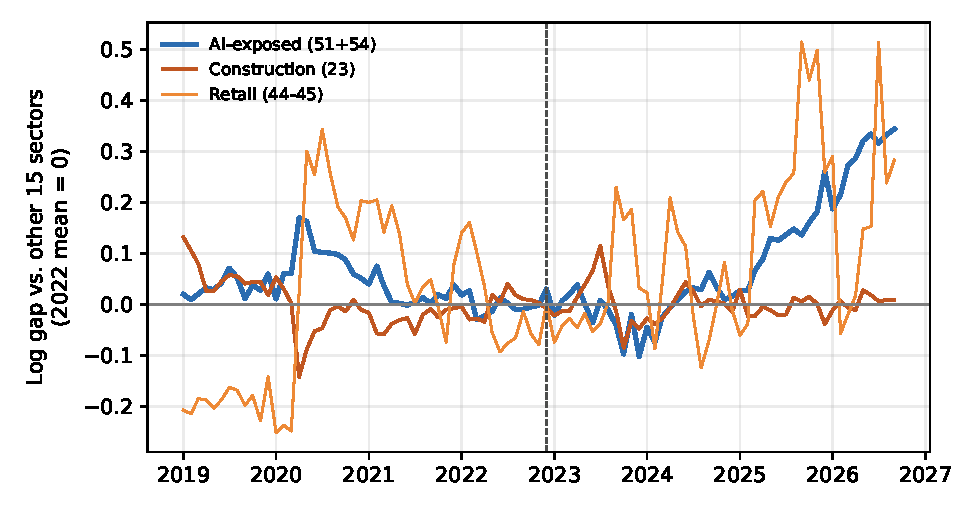
\includegraphics[width=0.85\linewidth]{bfs_monthly_gap}
  \caption{Business applications in AI-exposed sectors relative to other sectors.
    Log gap between seasonally adjusted monthly applications in each group and the mean of the 15 other NAICS sectors, normalized to the 2022 mean.
    AI-exposed is the mean of Information (51) and Professional services (54).
    Dashed line: December 2022.
    \footnotesize\textit{Source: Census BFS, January 2019--September 2026; our calculations.}}
  \label{fig:bfs-gap}
\end{figure}

\begin{table}[t]
  \centering
  \caption{Pre-trend, placebo and permutation tests: log business applications}
  \label{tab:bfs-tests}
  \begin{tabular}{lcccc}
    \toprule
     & Pre-trend & Fake shock & Event coef. & Rank of 2026 \\
     & 2010--22 (\%/yr) & 2016 & 2026 & among 171 pairs \\
    \midrule
    \multicolumn{5}{l}{\textit{All applications}} \\
    Information + Professional (51, 54) & $-0.26$ \, (1.0) & $-0.001$ \, (0.053) & $0.292$ \, (0.059) & 10 \\
    Placebo: Construction (23)          & $2.26$           & $0.189$              & $0.005$              & -- \\
    Placebo: Retail (44--45)            & $3.81$           & $0.093$              & $0.187$              & -- \\
    \multicolumn{5}{l}{\textit{High-propensity applications}} \\
    Information + Professional (51, 54) & $-0.21$ \, (1.0) & $0.020$ \, (0.058)  & $0.116$ \, (0.124)  & 48 \\
    \bottomrule
  \end{tabular}
  \par\smallskip
  \parbox{\linewidth}{\footnotesize Two-way (sector, year) fixed effects; controls are the 15 other NAICS sectors; base year 2022; 2026 is January--September.
    Standard errors clustered by sector in parentheses (reported for the two-sector group only).
    Fake shock: 2016--2019 vs.\ 2010--2015.
    Rank: position of the group's 2026 gap (relative to 2022, against the other 17 sectors) among all $\binom{19}{2} = 171$ sector pairs, 1 = largest.
    \textit{Source: Census BFS; our calculations.}}
\end{table}
